% !TEX encoding = UTF-8
% !TEX TS-program = pdflatex
% !TEX root = ../arsclassica.tex
% !TEX spellcheck = it-IT

%************************************************
\chapter{Esperimenti numerici}\label{cap:esperimenti}
%************************************************
\omissis{}
% introdurre argomenti del capitolo (dataset, e quindi tsis + sperimentazione)
% introdurre modalità di sperimentazione
% introdurre cross-validation
% spiegare metriche di valutazione utilizzate? si! ma in capitolo 4!

\section{\Ds{1}}\label{sec:dataset-1}
Lo scopo di questa sezione è presentare il \ds{1} e i risultati di classificazione e apprendimento strutturale ottenuti (si vedano rispettivamente i~\vref{cap:ctbnc,cap:structurallearning}) utilizzando tale insieme di \emph{\keyword{dati completi}} come input.

\subsection{Modello TSIS}\label{subsec:tsis-simple-model}
Al fine di introdurre il \ds{1} è necessario presentare la rete stradale \acs{TSIS} e il relativo modello di simulazione \acs{CORSIM} da cui esso è stato generato.

La~\vref{fig:tsis-model-simple} mostra la rete stradale che compone il modello \acs{TSIS} oggetto di questa sottosezione. Tale figura evidenzia:
\begin{itemize}
	\item la disposizione dei sensori utilizzati per il monitoraggio del passaggio dei veicoli
	\item le strade, tutte composte da $2$ corsie, e le intersezioni da cui è composta la rete stradale
\end{itemize}
 
\begin{figure}[H]
  	\centering
  	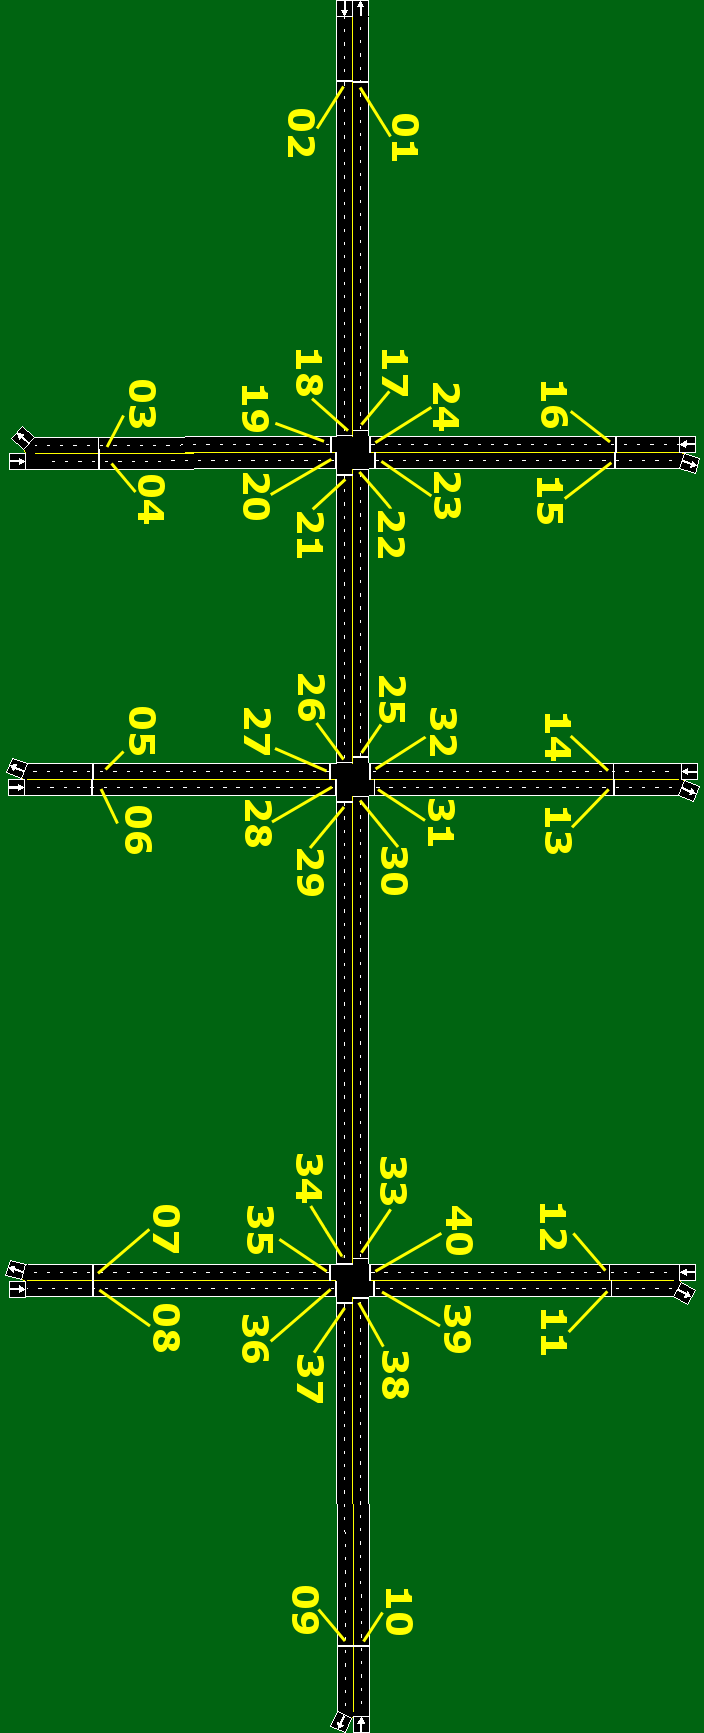
\includegraphics[max size={\textwidth}{\textheight}]{tsis-model-simple}% 
  	\caption[Rete stradale del \ds{1}]{Visualizzazione del file \acs{TNO} rappresentante la rete stradale da cui viene generato il \ds{1}. I sensori sono etichettati tramite degli indici numerici di colore giallo mentre le intersezioni (\ie{} nodi) sono etichettate tramite degli indici numerici di colore bianco.}
	\label{fig:tsis-model-simple}
\end{figure}


\begin{table}[htbp]%
	\centering%
	\begin{tabular}{+l^l}
	\toprule\rowstyle{\bfseries}%
	\# & Sensore  \\\otoprule
	$01$& D$212$\\
	$02$& D$121$\\
	$03$& D$272$\\
	$04$& D$721$\\
	$05$& D$392$\\
	$06$& D$931$\\
	$07$& D$4412$\\
	$08$& D$1141$\\
	$09$& D$452$\\
	$10$& D$541$\\\bottomrule
	\end{tabular}
	\hspace{-0.6em}
	\begin{tabular}{+l^l}
	\toprule\rowstyle{\bfseries}%
	\# & Sensore  \\\otoprule
	$11$& D$4102$\\
	$12$& D$1041$\\
	$13$& D$382$\\
	$14$& D$831$\\
	$15$& D$262$\\
	$16$& D$621$\\
	$17$& D$211$\\
	$18$& D$122$\\
	$19$& D$271$\\
	$20$& D$722$\\\bottomrule
	\end{tabular}
	\hspace{-0.6em}
	\begin{tabular}{+l^l}
	\toprule\rowstyle{\bfseries}%
	\# & Sensore  \\\otoprule
	$21$& D$231$\\
	$22$& D$322$\\
	$23$& D$261$\\
	$24$& D$622$\\
	$25$& D$321$\\
	$26$& D$232$\\
	$27$& D$391$\\
	$28$& D$932$\\
	$29$& D$341$\\
	$30$& D$432$\\\bottomrule
	\end{tabular}
	\hspace{-0.6em}
	\begin{tabular}{+l^l}
	\toprule\rowstyle{\bfseries}%
	\# & Sensore  \\\otoprule
	$31$& D$381$\\
	$32$& D$832$\\
	$33$& D$431$\\
	$34$& D$342$\\
	$35$& D$4111$\\
	$36$& D$1142$\\
	$37$& D$451$\\
	$38$& D$542$\\
	$39$& D$4101$\\
	$40$& D$1042$\\\bottomrule
	\end{tabular}
	\caption[Sensori del \ds{1}]{Corrispondenza fra gli identificatori dei sensori del \ds{1} e l'indice con cui essi sono indicati nella~\autoref{fig:tsis-model-simple}.}
	\label{tab:ds-1-sensors-indices}
\end{table}

%immagine piano semaforico? no
%dire che ci sono (e dove sono) i semafori (l'immagine non li contiene), al massimo incollarli sull'immagine ...
%spiegare come è fatta la rete stradale e modello di simulazione del traffico: time period, semafori, come va il traffico durante i time period

\subsection{Risultati}
\omissis{}
Prova~\vref{fig:tsis-model-monza-nodes} ...

%see: https://gist.github.com/leodido/5990626

\section{\Ds{2}}\label{sec:dataset-2}
\omissis{}

\subsection{Modello TSIS}\label{subsec:tsis-monza-model}
\omissis{}

% dire che parte da uno studio già fatto con sensori reali, riprodotto in tsis e esteso con altri sensori da me

\begin{table}[htbp]%
	\centering%
	\begin{tabular}{+l^l^l^l}
	\toprule\rowstyle{\bfseries}%
	Fascia oraria  		   & Time Period  	& Fase          & Classe  \\\otoprule
	$00$:$00$ - $02$:$05$  & $1$            & notturna      & $1$     \\
	$02$:$05$ - $04$:$10$  & $2$            & notturna      & $1$     \\
	$04$:$10$ - $06$:$15$  & $3$            & alba          & $2$     \\
	$06$:$15$ - $08$:$20$  & $4$            & mattino       & $3$     \\
	$08$:$20$ - $10$:$25$  & $5$            & mattino       & $3$     \\
	$10$:$25$ - $12$:$30$  & $6$            & centrale      & $4$     \\
	$12$:$30$ - $14$:$35$  & $7$            & centrale      & $4$     \\
	$14$:$35$ - $16$:$40$  & $8$            & centrale      & $4$     \\
	$16$:$40$ - $18$:$45$  & $9$            & pomeridiana   & $5$     \\
	$18$:$45$ - $20$:$50$  & $10$           & pomeridiana   & $5$     \\
	$20$:$50$ - $22$:$55$  & $11$           & serale        & $6$     \\
	$22$:$55$ - $24$:$00$  & $12$           & serale        & $6$     \\\bottomrule
	\end{tabular}
	\caption[Periodi temporali del \ds{2}]{Caratterizzazione dei periodi temporali (\ie{} \emph{\keyword{time period}}) del modello \acs{TSIS} relativo al \ds{2}.}
	\label{tab:ds-2-tp-labels}
\end{table}
%Saturday classes: `11`, `12`, ..., `16`.

%\cleardoublepage
%\begin{center}
%\capfigure
%\captionsetup{type=figure}
%\captionsetup[subfigure]{labelformat=empty}
%\subfloat[]{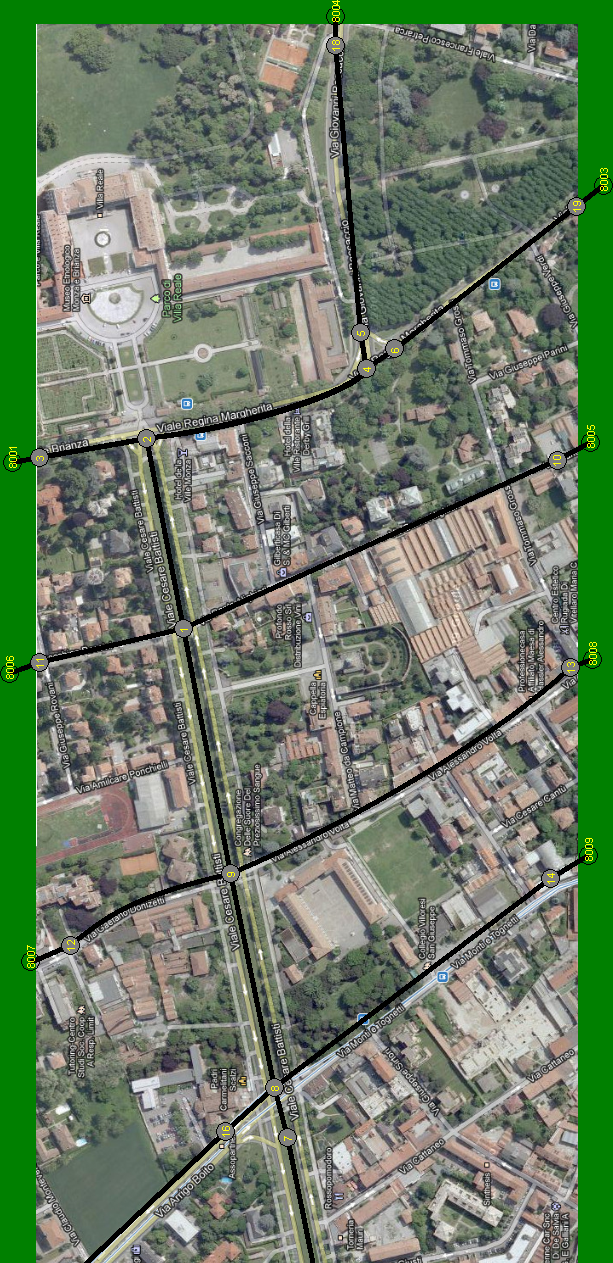
\includegraphics[width=1\columnwidth]{tsis-model-monza-gmap-dx}}\cleardoublepage
%\subfloat[]{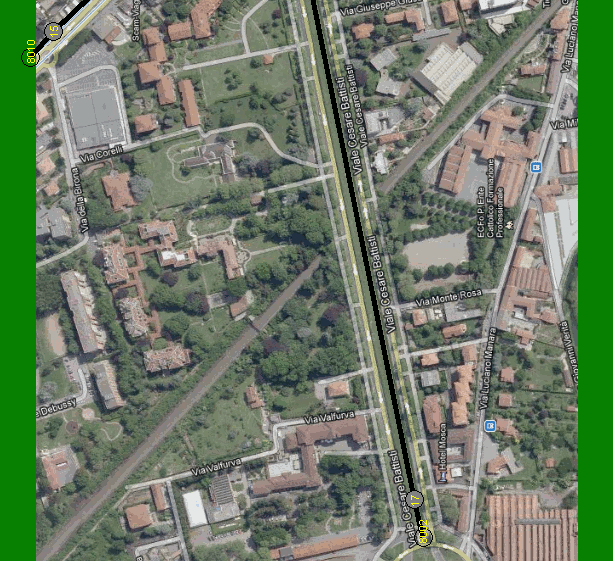
\includegraphics[width=1\columnwidth]{tsis-model-monza-gmap-sx}}
%\captionof{figure}[Intersezioni della rete stradale del \ds{2}]{Visualizzazione del file \acs{TNO} rappresentante le intersezioni della rete stradale da cui viene generato il \ds{2}.}
%\label{fig:tsis-model-monza-nodes}
%\end{center}

\begin{figure}[ht]
  \centering
  \captionsetup[subfigure]{labelformat=empty}
  \subfloat[][]{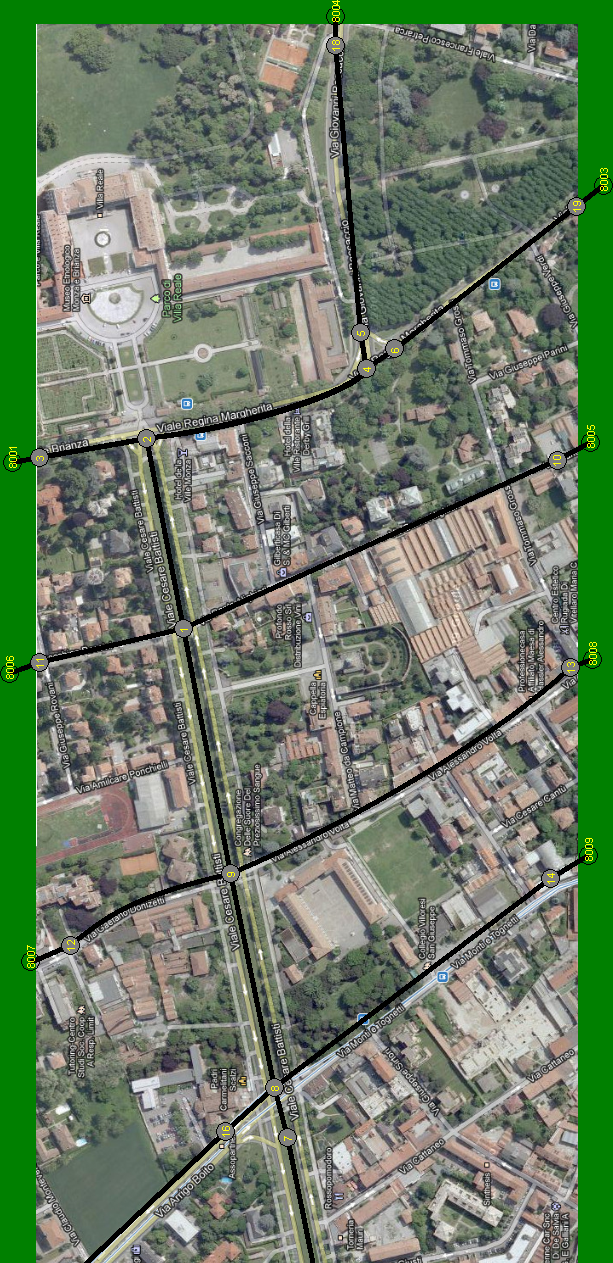
\includegraphics[width=0.935\columnwidth]{tsis-model-monza-gmap-dx}}%
  \phantomcaption
  \label{fig:tsis-model-monza-nodes}
\end{figure}
\begin{figure}[!t]
  \centering
  \captionsetup{type=figure}
  \captionsetup[subfigure]{labelformat=empty}
  \subfloat[][]{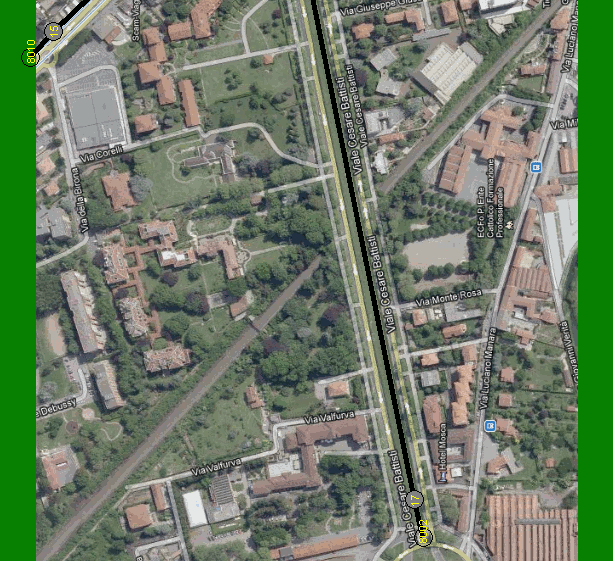
\includegraphics[width=0.935\columnwidth]{tsis-model-monza-gmap-sx}}% 
  \caption[Intersezioni della rete stradale del \ds{2}]{Visualizzazione del file \acs{TNO} rappresentante le intersezioni della rete stradale da cui viene generato il \ds{2}.}
\end{figure} 

\begin{table}[htbp]%
	\centering%
	\begin{tabular}{+l^l}
	\toprule\rowstyle{\bfseries}%
	Nodo    & Nome intersezione/strada\\\otoprule
	$1$     & dante                 \\
	$2$     & villa                 \\
	$3$     & viale brianza         \\
	$4$     & boccaccio             \\
	$5$     & via boccaccio         \\
	$6$     & p.zza citterio        \\
	$7$     & viale cesare battisti \\
	$8$     & boito                 \\
	$9$     & volta                 \\
	$10$    & via dante alighieri   \\
	$11$    & via g. rossini        \\
	$12$    & via donizzetti        \\
	$13$    & via a. volta          \\
	$14$    & via tognetti          \\
	$16$    & via boito             \\\bottomrule
	\end{tabular}
	\caption[Intersezioni del \ds{2}]{Caratterizzazione degli identificatori delle intersezioni (o nodi) del \ds{2}.}
	\label{tab:ds-2-nodes}
\end{table}

% inserire nomi vie visibili
\begin{figure}[ht]
  	\centering
  	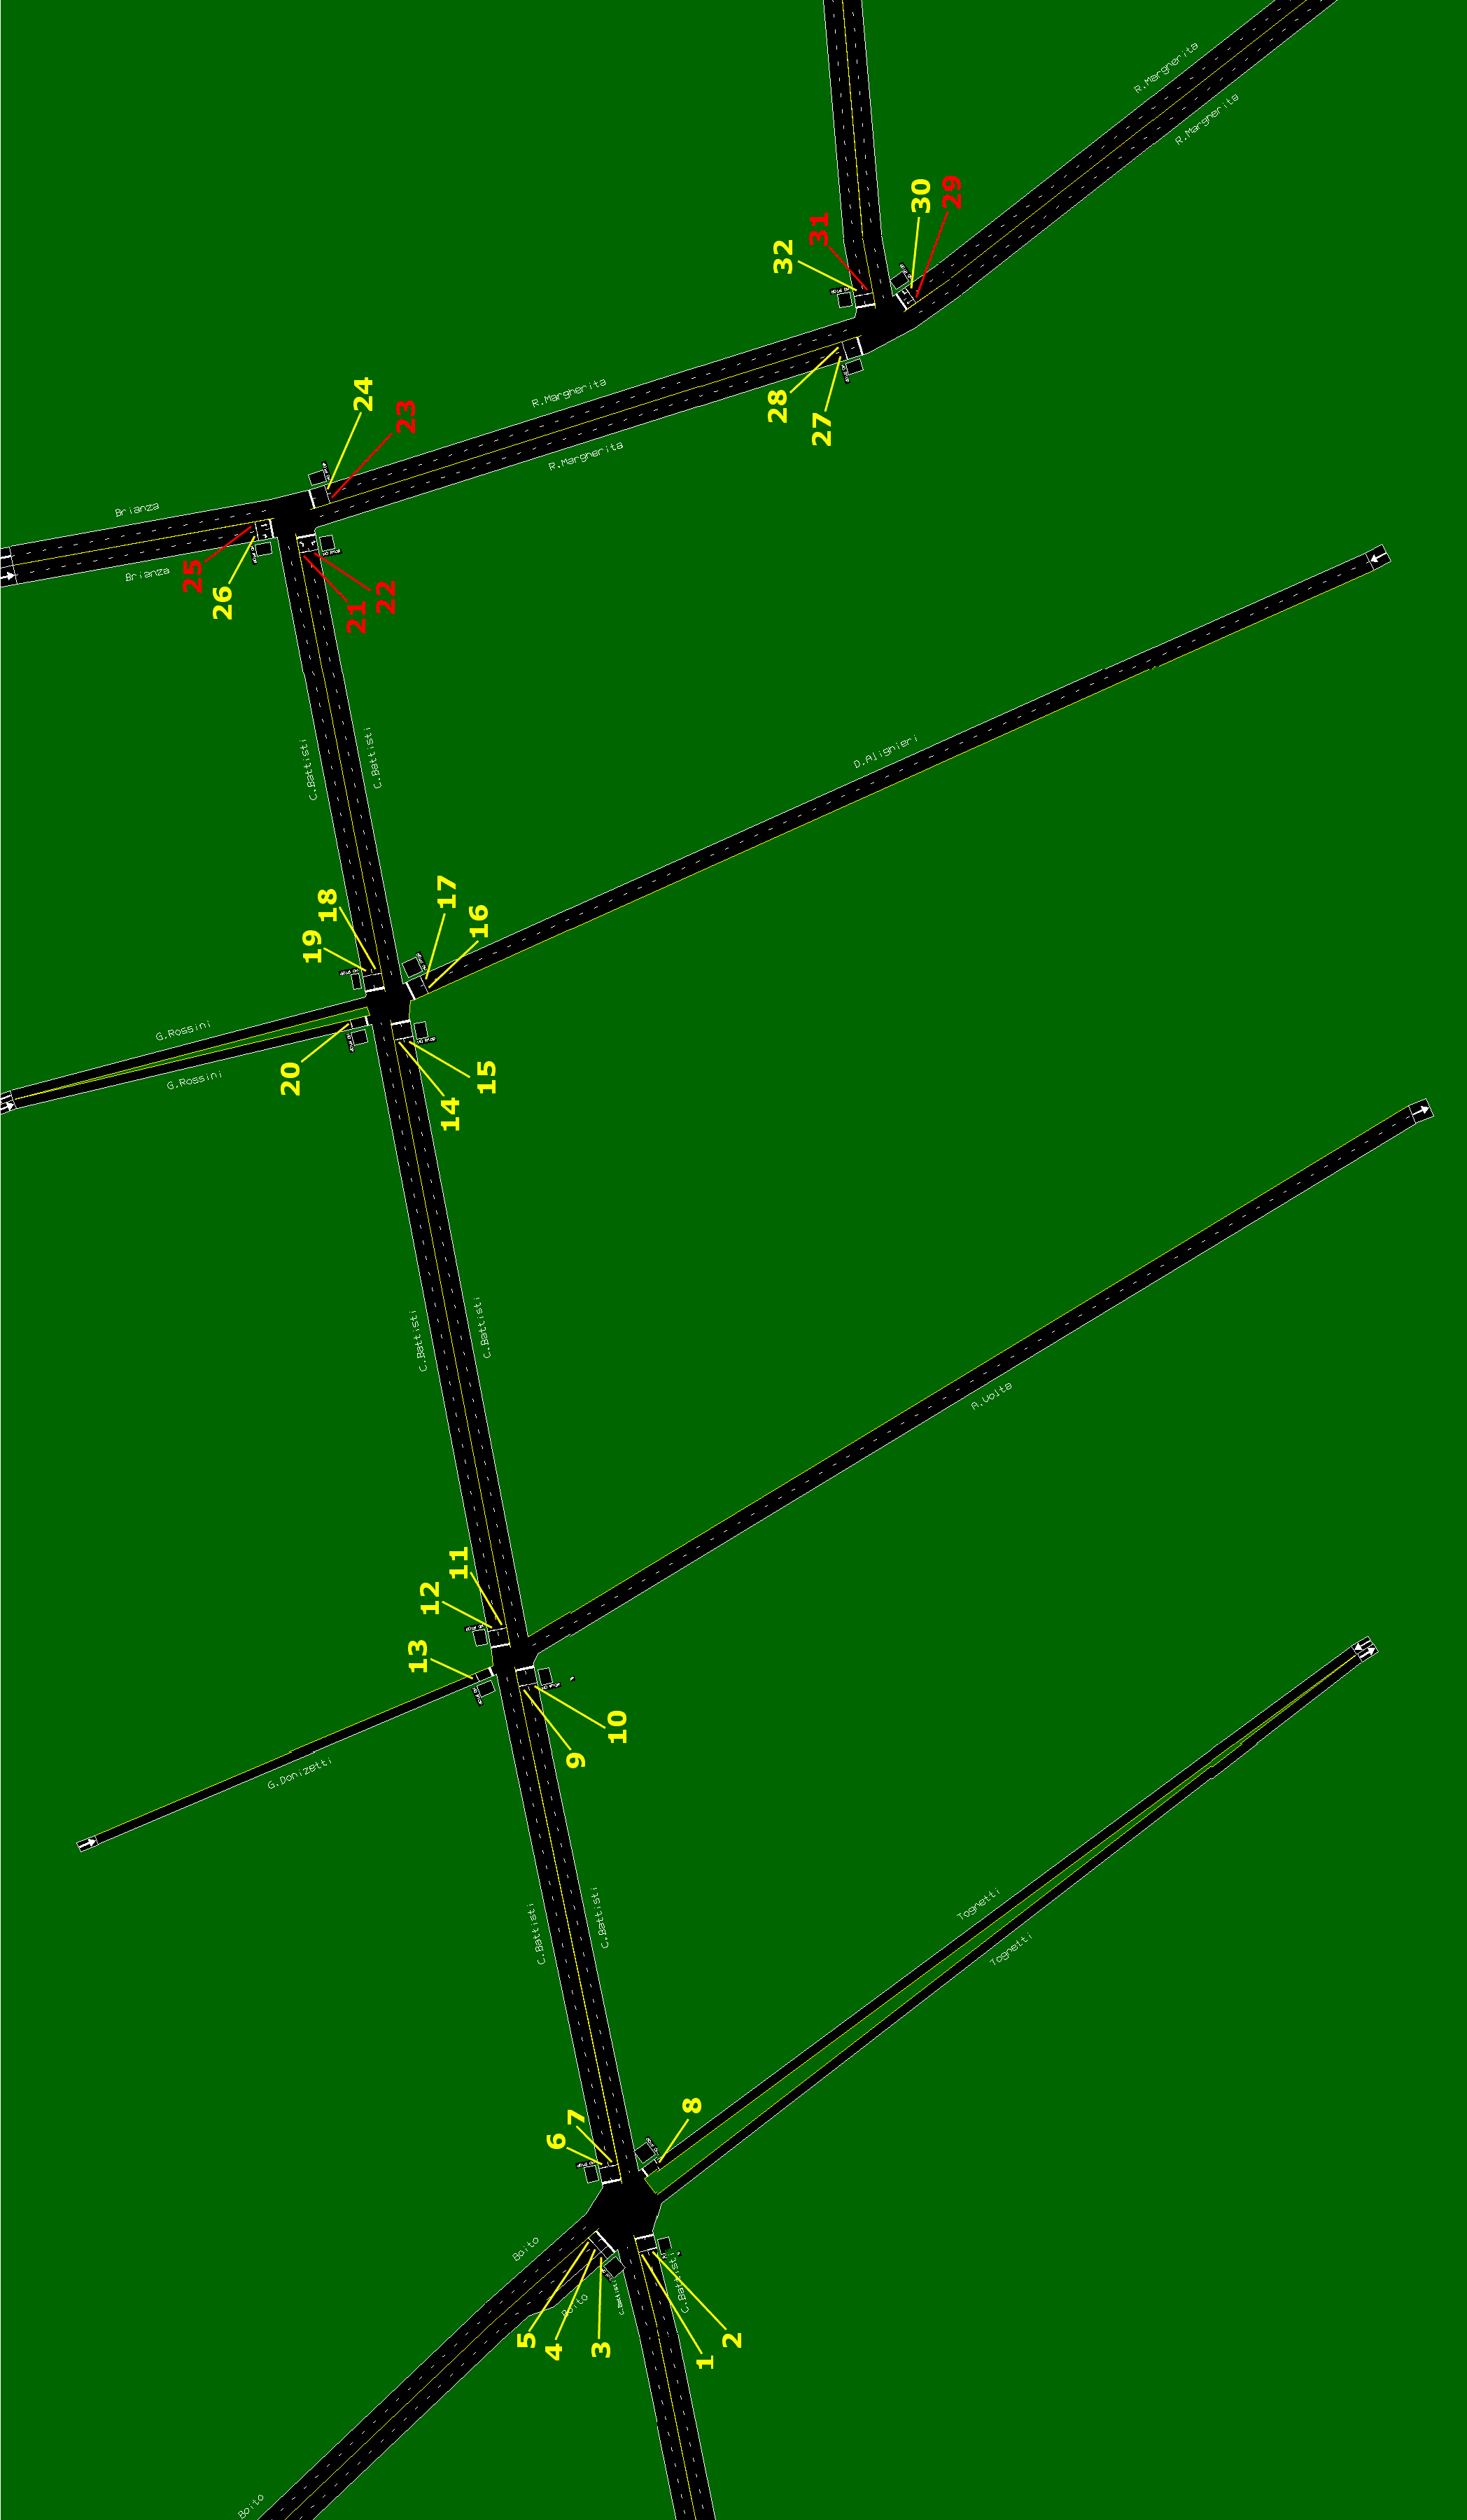
\includegraphics[width=1\columnwidth]{tsis-model-monza-compact}% 
  	\caption[Rete stradale del \ds{2}]{Visualizzazione del file \acs{TNO} rappresentante la rete stradale da cui viene generato il \ds{2}.}
	\label{fig:tsis-model-monza}
\end{figure} 

%TODO: migliorare ..
Di seguito si elencano le informazioni dei sensori reali del modello in questione:
\begin{description}
\item[$5094$] \hfill \\
Rilevamento dei veicoli provenienti da P.zza Citterio.
\item[$5095$] \hfill \\
Rilevamento dei veicoli provenienti dall'intersezione \virgolette{Boccaccio} diretti verso il centro di Monza.
\item[$5096$] \hfill \\
Rilevamento dei veicoli provenienti da Brianza verso Vedano.
\item[$5097$] \hfill \\
Rilevamento dei veicoli provenienti Regina Margherita che svoltano a sinistra in Battisti.
\item[$5098$] \hfill \\
Rilevamento dei veicoli provenienti da Battisti che svoltano a sinistra verso Vedano.
\item[$5099$] \hfill \\
Rilevamento dei veicoli provenienti da Battisti diretti verso il centro di Monza.
\end{description}

I sensori non reali aggiunti alla rete stradale che simula questa situazione di traffico reale vengono identificati secondo uno schema ben preciso. Il loro identificatore è composto in base al senso di marcia. Nello specifico tale numero è una concatenazione dei seguenti valori: identificatore dell'intersezione di partenza, identificatore dell'intersezione d'arrivo, numero indicante la corsia su cui il sensore è posto (\ie{} $0$ se è la strada possiede una sola corsia, $1$ o $2$ se il sensore è posto rispettivamente a destra o a sinitra, $7$ o $8$ nel caso in cui esso sia posto su ulteriori corsie di destra o sinistra). Ad esempio:
\begin{itemize}
\item il sensore identificato da D$912$ è posto sulla corsia di sinistra della strada che collega l'intersezione \virgolette{Volta} (\ie{} nodo $9$) all'intersezione \virgolette{Dante} (\ie{} nodo $1$)
\item il sensore identificato da D$1480$ è posto sull'unica corsia di \virgolette{Via Tognetti} (\ie{} nodo $14$) nei pressi dell'incrocio con l'intersezione \virgolette{Boito} (\ie{} nodo $8$).
\end{itemize}

\begin{table}[htbp]%
	\centering%
	\begin{tabular}{+l^l}
	\toprule\rowstyle{\bfseries}%
	\#  & Sensore \\\otoprule
	$01$& D$782$       \\
	$02$& D$781$       \\
	$03$& D$1687$      \\
	$04$& D$1681$      \\
	$05$& D$1682$      \\
	$06$& D$981$       \\
	$07$& D$982$       \\
	$08$& D$1480$      \\\bottomrule
	\end{tabular}
	\hspace{-0.6em}
	\begin{tabular}{+l^l}
	\toprule\rowstyle{\bfseries}%
	\#  & Sensore \\\otoprule
	$09$& D$892$       \\
	$10$& D$891$       \\
	$11$& D$192$       \\
	$12$& D$191$       \\
	$13$& D$1290$      \\
	$14$& D$912$       \\
	$15$& D$911$       \\
	$16$& D$1092$      \\\bottomrule
	\end{tabular}
	\hspace{-0.6em}
	\begin{tabular}{+l^l}
	\toprule\rowstyle{\bfseries}%
	\#  & Sensore \\\otoprule
	$17$& D$1091$      \\
	$18$& D$212$       \\
	$19$& D$211$       \\
	$20$& D$110$       \\
	\color{red}$21$& D$5098*$     \\
	\color{red}$22$& D$5099*$     \\
	\color{red}$23$& D$5097*$     \\
	$24$& D$421$       \\\bottomrule
	\end{tabular}
	\hspace{-0.6em}
	\begin{tabular}{+l^l}
	\toprule\rowstyle{\bfseries}%
	\#  & Sensore \\\otoprule
	\color{red}$25$& D$5096*$     \\
	$26$& D$321$       \\
	$27$& D$241$       \\
	$28$& D$242$       \\
	\color{red}$29$& D$5094*$     \\
	$30$& D$642$       \\
	\color{red}$31$& D$5095*$     \\
	$32$& D$541$       \\\bottomrule
	\end{tabular}
	\caption[Sensori del \ds{2}]{Corrispondenza fra gli identificatori dei sensori del \ds{2} e l'indice con cui essi sono indicati nella \omissis{}}
	\label{tab:ds-2-sensors-indices}
\end{table}

Nella~\vref{tab:ds-2-sensors-indices}, i sensori il cui identificatore è contrassegnato da un asterisco corrispondono ai sensori reali, evidenziati anche nella figura \omissis{} tramite un indice numerico di colore rosso.

%varianti del dataset utilizzate
%split figure on more pages (search google is my friend)

\subsection{Risultati}
\omissis{}



%see: https://gist.github.com/leodido/5733991

%risultati:
%apprendimento
%classificazione (cross-validated)
%apprendimento strutturale (cross-validated)